\documentclass[10pt,a4paper]{article}

\usepackage[margin=19mm]{geometry}
\usepackage[T1]{fontenc}
\usepackage{lmodern}
\usepackage{xcolor}
\usepackage{booktabs}
\usepackage{longtable}
\usepackage{array}
\usepackage{graphicx}
\usepackage{tikz}
\usepackage{listings}
\usepackage{tcolorbox}
\usepackage{fancyhdr}
\usepackage{hyperref}
\usetikzlibrary{arrows.meta,positioning,shapes.geometric}

\definecolor{ink}{HTML}{172033}
\definecolor{blue}{HTML}{1D5D7A}
\definecolor{mint}{HTML}{DCEFE8}
\definecolor{amber}{HTML}{F7E4B5}
\definecolor{mist}{HTML}{F2F5F7}
\definecolor{codebg}{HTML}{F7F9FA}

\hypersetup{colorlinks=true,linkcolor=blue,urlcolor=blue,pdftitle={Vinglish Zero Deterministic Reasoning Showcase}}
\pagestyle{fancy}
\fancyhf{}
\lhead{Vinglish Zero}
\rhead{Deterministic Reasoning Showcase}
\cfoot{\thepage}
\setlength{\headheight}{14pt}

\lstdefinestyle{artifact}{
  basicstyle=\ttfamily\scriptsize,
  backgroundcolor=\color{codebg},
  frame=single,
  rulecolor=\color{blue!35},
  breaklines=true,
  breakatwhitespace=false,
  columns=fullflexible,
  showstringspaces=false,
  keepspaces=true,
  aboveskip=7pt,
  belowskip=7pt
}
\lstset{style=artifact}

\newcommand{\artifact}[2]{\paragraph{#1}\lstinputlisting{#2}}
\newcommand{\corecase}[2]{
  \subsection{#1}
  \artifact{Original source}{../gallery/#2/source.py}
  \artifact{Facts extracted}{../gallery/#2/facts.json}
  \artifact{Evidence produced}{../gallery/#2/evidence.json}
  \artifact{Remaining hypotheses and confidence}{../gallery/#2/remaining-hypotheses.json}
  \artifact{Constraint eliminations}{../gallery/#2/constraint-eliminations.json}
  \artifact{Final IntentReport}{../gallery/#2/intent-report.json}
  \noindent Full Semantic IR and direct rejected-evidence rendering are retained
  in the corresponding gallery directory.
}
\newcommand{\errorcase}[2]{
  \clearpage
  \subsection{#1}
  \artifact{Source}{../gallery/#2/source.py}
  \begingroup\tiny
  \lstinputlisting{../gallery/#2/error-gallery-card.txt}
  \endgroup
  \noindent The full compiler diagnostic, SemanticDiagnostic, suggestions, and
  constraint outputs are retained in the corresponding gallery directory.
}

\begin{document}

\pagenumbering{gobble}
\begin{titlepage}
\pagecolor{mist}
\color{ink}
\vspace*{28mm}
{\Huge\bfseries Vinglish Zero\\[3mm]}
{\LARGE Deterministic Reasoning and Semantic Diagnostics Showcase\par}
\vspace{12mm}
\begin{tcolorbox}[colback=mint,colframe=blue!65,boxrule=0.7pt]
This document is a capture of the canonical implementation. It adds no
reasoning rules, no diagnostics rules, and no Semantic IR concepts. Every
fact, evidence item, hypothesis, elimination, confidence score, intent report,
and semantic diagnostic shown here is generated from the checked-in public APIs.
\end{tcolorbox}
\vfill
\begin{tabular}{@{}ll@{}}
Capture runner & \texttt{cargo run -p vz-adapter-python --example showcase} \\
Artifact root & \texttt{gallery/} \\
Languages exercised & Python standard AST and Vinglish transport v1 \\
Document source & \texttt{latex/showcase.tex}
\end{tabular}
\vspace*{18mm}
\end{titlepage}
\nopagecolor
\clearpage
\pagenumbering{arabic}

\tableofcontents
\clearpage

\section{Scope and Reproducibility}

The showcase is documentation and test data, not a feature change. The runner
uses the existing Python adapter, Vinglish transport adapter, FactExtractor,
ReasoningEngine, and SemanticDiagnosticEngine as published. It writes a source
file and all available artifacts for each case. Invalid syntax is retained as an
adapter error because no Semantic IR exists to reason over. Unsupported syntax
is retained as an analyzed graph if the adapter can construct one.

\begin{tcolorbox}[colback=amber!38,colframe=amber!70!black,title=Diagnostic input boundary]
Python has no compiler-diagnostic exporter in the current repository. The
error-gallery diagnostic objects are explicit instances of the existing
language-neutral \texttt{CompilerDiagnostic} model. The semantic diagnostic
output is real; the diagnostic input is clearly captured beside it. No compiler
behavior is claimed for Python.
\end{tcolorbox}

\section{Architecture Overview}

\begin{center}
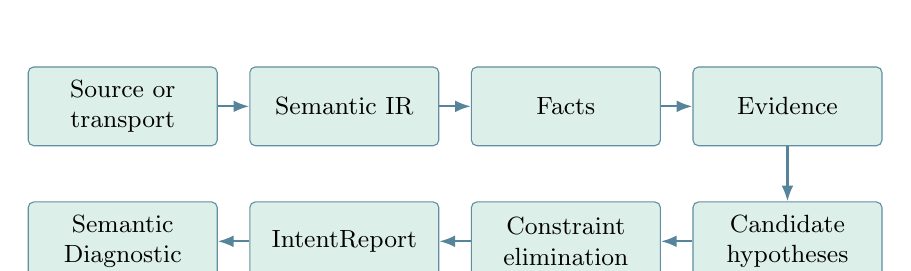
\begin{tikzpicture}[
  node distance=7mm and 4mm,
  box/.style={draw=blue!70,rounded corners=2pt,fill=mint,minimum width=24mm,minimum height=10mm,align=center,font=\small},
  arrow/.style={-{Latex[length=2mm]},thick,draw=blue!75}
]
\node[box] (source) {Source or\\transport};
\node[box,right=of source] (ir) {Semantic IR};
\node[box,right=of ir] (facts) {Facts};
\node[box,right=of facts] (evidence) {Evidence};
\node[box,below=of evidence] (hypotheses) {Candidate\\hypotheses};
\node[box,left=of hypotheses] (constraints) {Constraint\\elimination};
\node[box,left=of constraints] (intent) {IntentReport};
\node[box,left=of intent] (diagnostic) {Semantic\\Diagnostic};
\draw[arrow] (source) -- (ir);
\draw[arrow] (ir) -- (facts);
\draw[arrow] (facts) -- (evidence);
\draw[arrow] (evidence) -- (hypotheses);
\draw[arrow] (hypotheses) -- (constraints);
\draw[arrow] (constraints) -- (intent);
\draw[arrow] (intent) -- (diagnostic);
\end{tikzpicture}
\end{center}

\subsection{Evidence and rule flow}
\begin{center}
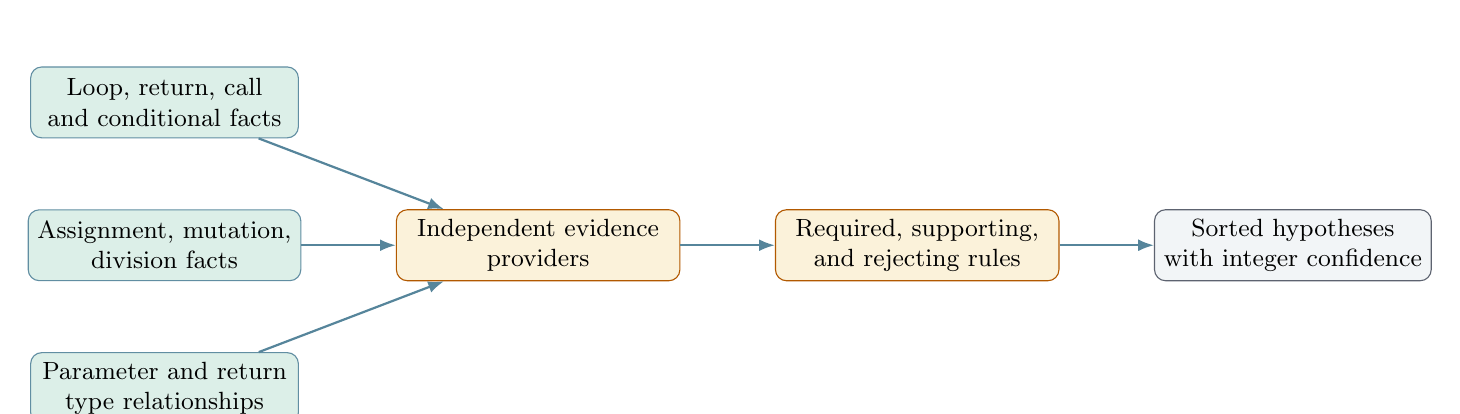
\begin{tikzpicture}[
  node distance=9mm and 12mm,
  source/.style={draw=blue!70,fill=mint,rounded corners,minimum width=34mm,minimum height=9mm,align=center,font=\small},
  rule/.style={draw=orange!70!black,fill=amber!50,rounded corners,minimum width=36mm,minimum height=9mm,align=center,font=\small},
  outcome/.style={draw=ink!70,fill=mist,rounded corners,minimum width=33mm,minimum height=9mm,align=center,font=\small},
  arrow/.style={-{Latex[length=2mm]},thick,draw=blue!75}
]
\node[source] (flow) {Loop, return, call\\and conditional facts};
\node[source,below=of flow] (mutation) {Assignment, mutation,\\division facts};
\node[source,below=of mutation] (type) {Parameter and return\\type relationships};
\node[rule,right=of mutation] (providers) {Independent evidence\\providers};
\node[rule,right=of providers] (rules) {Required, supporting,\\and rejecting rules};
\node[outcome,right=of rules] (report) {Sorted hypotheses\\with integer confidence};
\draw[arrow] (flow) -- (providers);
\draw[arrow] (mutation) -- (providers);
\draw[arrow] (type) -- (providers);
\draw[arrow] (providers) -- (rules);
\draw[arrow] (rules) -- (report);
\end{tikzpicture}
\end{center}

\subsection{Constraint evaluation example}
\begin{center}
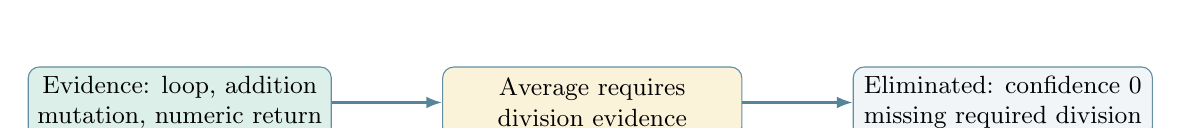
\begin{tikzpicture}[
  node distance=8mm and 14mm,
  box/.style={draw=blue!70,rounded corners,minimum width=38mm,minimum height=9mm,align=center,font=\small},
  arrow/.style={-{Latex[length=2mm]},thick,draw=blue!75}
]
\node[box,fill=mint] (ev) {Evidence: loop, addition\\mutation, numeric return};
\node[box,fill=amber!50,right=of ev] (rule) {Average requires\\division evidence};
\node[box,fill=mist,right=of rule] (out) {Eliminated: confidence 0\\missing required division};
\draw[arrow] (ev) -- (rule);
\draw[arrow] (rule) -- (out);
\end{tikzpicture}
\end{center}

\section{Capture Inventory}

\artifact{Complete index of generated cases}{../gallery/index.json}

Each analyzed case has the following direct artifacts:
\begin{center}
\begin{tabular}{@{}p{38mm}p{104mm}@{}}
\toprule
Artifact & Content \\
\midrule
\texttt{source.py} or \texttt{transport.json} & Original input captured by the runner. \\
\texttt{semantic-ir.debug.txt} & Adapter-produced SemanticGraph debug representation. \\
\texttt{facts.json} & Immutable FactExtractor result. \\
\texttt{evidence.json} & Evidence collected for each function. \\
\texttt{candidate-hypotheses.json} & Every candidate, including active and eliminated results. \\
\texttt{constraint-eliminations.json} & Eliminated candidates with exact rejected-evidence records. \\
\texttt{remaining-hypotheses.json} & Active candidates only. \\
\texttt{confidence-scores.json} & Candidate IDs, statuses, and confidence values. \\
\texttt{intent-report.json} & Canonical reasoning output. \\
\texttt{semantic-diagnostic.json} & Existing diagnostics output where a diagnostic input was supplied. \\
\bottomrule
\end{tabular}
\end{center}

\section{Example Gallery}

The following representative cases show original inputs and the complete
public reasoning artifacts. Their companion directories contain the full
Semantic IR debug representation and direct rejected-evidence rendering.

\corecase{Accumulator}{accumulator}
\corecase{Counter}{counter}
\corecase{Average}{average}
\corecase{Mapper}{mapper}
\corecase{Filter}{filter}
\corecase{Validator}{validator}
\corecase{State Machine}{state_machine}
\corecase{Nested Loops}{nested_loops}
\corecase{Recursion}{recursion}
\corecase{Unsupported Pattern Matching}{pattern_matching}

\section{Error Gallery}

Each error-gallery card is a compact direct rendering of the source, supplied
compiler diagnostic, selected intent, evidence, confidence, semantic diagnostic,
suggested fixes, and every rejected hypothesis. It contains no generated prose.

\errorcase{Accumulator Type Mismatch}{accumulator}
\errorcase{Average Missing Division}{missing_division}
\errorcase{Ownership-style Move After Use}{ownership}
\errorcase{Wrong Return Type}{wrong_return_type}
\errorcase{Incorrect Accumulator}{incorrect_accumulator}

\section{Cross-language Comparison}

The Python accumulator and the Vinglish v1 transport fixture use independent
adapters. The following two actual report projections demonstrate that the
downstream reasoning output is based on Semantic IR rather than source language.

\artifact{Python accumulator active hypotheses}{../gallery/accumulator/remaining-hypotheses.json}
\artifact{Vinglish transport accumulator active hypotheses}{../gallery/cross_language_vinglish_accumulator/remaining-hypotheses.json}

\section{Determinism Verification}

Selected valid examples are run five times. The runner serializes each
IntentReport and, where supplied, each SemanticDiagnostic to bytes and asserts
byte identity before writing these results. The check covers arithmetic, counter,
filter, nested loops, unsupported pattern matching, both accumulator diagnostics,
missing division, wrong return type, ownership-style move-after-use, and the
Vinglish transport accumulator.

\artifact{Accumulator determinism result}{../gallery/accumulator/determinism.json}
\artifact{Missing division determinism result}{../gallery/missing_division/determinism.json}
\artifact{Vinglish transport determinism result}{../gallery/cross_language_vinglish_accumulator/determinism.json}

\section{Performance and Distribution}

The timing capture is local wall-clock measurement in microseconds. It is not a
benchmark; its purpose is to document the observed run and expose the largest
example, most evidence, candidate volume, average confidence, and hypothesis
status distribution.

\artifact{Observed statistics}{../gallery/statistics.json}

\section{Unsupported and Malformed Inputs}

\subsection{Pattern matching}
The currently supported Python subset does not lower \texttt{match}. The
adapter still produces a function graph, but its body has no supported semantic
nodes. The resulting facts and all eliminated candidates are captured below.
\artifact{Pattern matching facts}{../gallery/pattern_matching/facts.json}
\artifact{Pattern matching eliminations}{../gallery/pattern_matching/constraint-eliminations.json}

\subsection{Malformed source}
Malformed input fails at Python AST parsing and therefore has no Semantic IR,
facts, evidence, intent report, or semantic diagnostic. This is an adapter
boundary outcome, not a reasoning-engine result.
\artifact{Malformed source}{../gallery/malformed_input/source.py}
\artifact{Adapter error}{../gallery/malformed_input/adapter-error.txt}

\section{Appendix: Full Artifact Map}

\artifact{Generated artifact index}{../gallery/index.json}

The generated \texttt{gallery/} tree is the complete machine-readable appendix.
For every analyzed example it includes the source, Semantic IR debug output,
facts, evidence, all candidates, eliminations, active hypotheses, confidences,
IntentReport, diagnostic output, suggestions, and direct rejected-evidence
rendering. This document intentionally includes representative full listings
and compact error cards to remain navigable while retaining all raw outputs
alongside it.

\end{document}
